\documentclass[11pt,a4paper]{article}
\usepackage[margin=2.2cm]{geometry}
\usepackage{booktabs}
\usepackage{tabularx}
\usepackage{array}
\usepackage{bytefield}
\usepackage{tikz}
\usetikzlibrary{positioning,arrows.meta}
\usepackage{xcolor}
\usepackage{enumitem}
\usepackage{amsmath}
\usepackage[hidelinks]{hyperref}
\usepackage{fancyhdr}
\usepackage{listings}
\lstset{basicstyle=\ttfamily\small,columns=fullflexible,keepspaces=true,frame=single,rulecolor=\color{gray}}

\definecolor{newc}{HTML}{0F6E56}
\newcommand{\new}{\textcolor{newc}{\textsf{\small NEW}}}
\definecolor{fivec}{HTML}{1D4ED8}
\newcommand{\vfive}{\textcolor{fivec}{\textsf{\small v0.5}}}
\definecolor{sixc}{HTML}{B45309}
\newcommand{\vsix}{\textcolor{sixc}{\textsf{\small v0.6}}}
\definecolor{sevenc}{HTML}{9D174D}
\newcommand{\vseven}{\textcolor{sevenc}{\textsf{\small v0.7}}}
\newcommand{\sig}[1]{\texttt{#1}}
\setlist{itemsep=2pt,topsep=4pt}
\setlength{\parskip}{4pt}
\setlength{\parindent}{0pt}

\pagestyle{fancy}
\fancyhf{}
\lhead{\small Paul Vincent Bezzina \textbar{} ProEm - Open Source Protocol Emulator}
\rhead{\small ISA draft v0.7.1}
\cfoot{\small\thepage}

\title{ProEm Instruction Set\\\large Draft v0.7.1}
\author{Paul Vincent Bezzina}
\date{13 October 2026}

\begin{document}
\maketitle

\section{Summary}

The RP2040 programs the emulator with a short list of byte instructions. The control unit decodes each instruction into one write of the frame chain's configuration registers (\sig{cfg\_*}); there is no instruction memory and nothing is replayed after reset. A program describes one frame: which block comes first, how many bits each block handles, which way each block talks, and what ends the frame. A \sig{RUN} instruction then starts it.

Everything in this draft is implemented in the RTL and tested end to end at pin level: each test sends instruction bytes to the chip, drives or models the protocol's real lines, and reads the results back over the return UART. v0.4 adds the line codec behind \sig{LINE} and \sig{CLOCK}, the \sig{OUT} and \sig{LINK} instructions, auto-baud and the return link (Section~\ref{sec:changes}). The changes from 25 September:

\begin{enumerate}
\item \textbf{Block index and direction in every block instruction.} Each instruction names the block it configures (\sig{HDR 1}, \sig{HDR 2}, \ldots) and carries its direction bit (0 = read, 1 = write). This is how the RTL already works internally; the ISA now makes it explicit.
\item \textbf{Run modes and block groups} \new. Each block is tagged \emph{always}, \emph{read only} or \emph{write only}. \sig{RUN READ} runs the \emph{always} and \emph{read only} blocks; \sig{RUN WRITE} runs the \emph{always} and \emph{write only} blocks. One program then covers both an I\textsuperscript{2}C register read and a register write.
\item \textbf{END pair compare} \new. END can combine two pins instead of watching one. With D+ and D$-$ this detects the USB end of packet (both low) and flags the illegal state (both high).
\item \textbf{Line decoding} \new. \sig{LINE} selects how a pin is decoded before the chain sees it: plain, NRZI (USB) or Manchester (10BASE-T), with optional bit unstuffing.
\item \textbf{Clock source} \new. \sig{CLOCK} selects where the chain's \sig{tick} comes from: SYNC (an input clock pin), ASYNC (an internal bit timer, as in a UART), generated by the chip on an output pin, or recovered by the line decoder.
\end{enumerate}

Items marked \new{} were added in v0.4 (25 September).

\paragraph{v0.5 (27 September).} Items marked \vfive{} are new in this version:
\begin{enumerate}
\item \textbf{\sig{BRANCH}} (\texttt{0xF}) \vfive: two rules per chain that change the frame's direction, or abort it, depending on a field the chain has just received, or on the line not reading back what the chip drove. This adds I\textsuperscript{2}C target mode, SWD-style acknowledge handling and CAN-style arbitration.
\item \textbf{Capture any value} \vfive: a read header with \sig{ANY} accepts whatever arrives and can return it, for fields such as the I\textsuperscript{2}C R/W bit, an SWD acknowledge or a USB PID.
\item \textbf{I\textsuperscript{2}C target} \vfive: with \sig{OUT I2C} and a SYNC clock the codec detects START, repeated START and STOP, and drives SDA only while SCL is low.
\item \textbf{Streaming and underrun} \vfive: \sig{DATA} can keep arriving while a write frame runs. On a line with fixed timing, running out of data aborts the frame and reports an underrun.
\item \textbf{Status byte} \vfive: bits 5--7 now report underrun, a branch match and a branch abort.
\end{enumerate}

\paragraph{v0.6 (11 October).} Items marked \vsix{} are new in this version:
\begin{enumerate}
\item \textbf{CRC on chip} \vsix: \sig{BRANCH 2} and \sig{BRANCH 3} set up one CRC per chain, any width from 1 to 16 bits and any polynomial. On a read frame the chain checks the CRC as the bits arrive and returns the result; on a write frame it appends the CRC after MAIN (Section~\ref{sec:crc}).
\item \textbf{Reply} \vsix: \sig{BRANCH 4} sends a short fixed pattern (up to 16 bits) a set number of bit times after a read frame ends, optionally only when the CRC was good or bad. This is the USB handshake (ACK) and the CAN acknowledge slot.
\item \textbf{Branch on the CRC} \vsix: a rule with \sig{SRC} = 1 and \sig{BLOCK} = 1 acts on the CRC result.
\item \textbf{CAN bit stuffing tested} \vsix: \sig{LINE} \sig{STUFF} = 5 with \sig{SANY} = 1 now has end-to-end tests, receive and chip to chip.
\end{enumerate}

\paragraph{v0.7 (11 October).} Items marked \vseven{} are new in this version. They remove the limits found while testing fifteen further standards; every field was reserved before, so v0.6 programs work unchanged.
\begin{enumerate}
\item \textbf{22-bit divider} \vseven: \sig{CLOCK} byte 2 bits 5--0 are \sig{DIV[21:16]}. The slowest rate at 50\,MHz falls from 763 to 12\,bit/s (RC5 infrared, K-Line 5-baud init).
\item \textbf{Manchester boundary lock} \vseven: \sig{LINE} byte 1 bit 3, \sig{BND}, makes the decoder treat the first edge after idle as a bit boundary (DALI, whose start bit begins with a boundary edge).
\item \textbf{Seeking headers} \vseven: \sig{HDR} byte 2 bit 5, \sig{SEEK}, makes a read header skip incoming bits until its first bit appears, so a frame can wait out a gap of any length, for example idle time before a start bit (LIN inter-byte space).
\item \textbf{Byte-field CRCs} \vseven: \sig{BRANCH 3} byte 1 bits 3 and 2, \sig{BYTE} and \sig{SPAN}, let the CRC skip fields shorter than 8 bits and run across frames (Modbus RTU, SMBus PEC).
\item \textbf{Release while reading} \vseven: with \sig{DRIVE} = \texttt{01} the data and pair outputs are released during generated read bits and between entries of a generated-clock frame, so one push-pull line can carry both directions (3-wire SPI, MDIO).
\end{enumerate}

\section{Frame chain recap}

\begin{center}
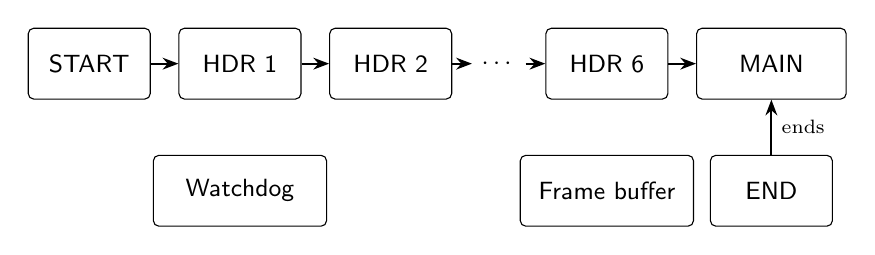
\begin{tikzpicture}[
  blk/.style={draw,rounded corners=2pt,minimum width=1.55cm,minimum height=0.9cm,font=\small\sffamily,align=center},
  arr/.style={-{Stealth[length=2mm]},thick}]
\node[blk] (s) {START};
\node[blk,right=0.35cm of s] (h1) {HDR 1};
\node[blk,right=0.35cm of h1] (h2) {HDR 2};
\node[right=0.25cm of h2,font=\small] (dots) {$\cdots$};
\node[blk,right=0.25cm of dots] (h6) {HDR 6};
\node[blk,right=0.35cm of h6,minimum width=1.9cm] (m) {MAIN};
\node[blk,below=0.7cm of m] (e) {END};
\node[blk,below=0.7cm of h1,minimum width=2.2cm] (w) {Watchdog};
\node[blk,below=0.7cm of h6,minimum width=2.2cm] (fb) {Frame buffer};
\draw[arr] (s) -- (h1); \draw[arr] (h1) -- (h2); \draw[arr] (h2) -- (dots); \draw[arr] (dots) -- (h6); \draw[arr] (h6) -- (m);
\draw[arr] (e) -- node[right,font=\scriptsize]{ends} (m);
\end{tikzpicture}
\end{center}

\begin{itemize}
\item Blocks run strictly in order, one bit per \sig{tick}. A block that is not configured (or, with groups, not active in this run) is skipped.
\item A \emph{read} block samples its pin on each tick and compares or captures. A mismatch aborts the frame.
\item A \emph{write} block pushes its value into the frame buffer as a \sig{wire} entry for the TX sender and succeeds in one clock.
\item Read blocks only take ticks once every written bit ahead of them has left the chip (\sig{line\_free}), so a frame can write a request and read the reply.
\item START and END have their own pins. The headers and MAIN share the data pin set by \sig{MAIN}.
\item Up to two chains (A and B) run side by side, for full-duplex SPI.
\end{itemize}

\section{Instruction format}

Every instruction starts with one byte: a 4-bit opcode and a 4-bit index. Operand bytes follow; multi-byte numbers are sent high byte first.

\begin{center}
\begin{bytefield}[bitwidth=2.4em]{8}
\bitheader[endianness=big]{0-7}\\
\bitbox{4}{\sig{OP}} & \bitbox{1}{\sig{CH}} & \bitbox{3}{\sig{N}}
\end{bytefield}
\end{center}

\sig{CH} selects chain A (0) or chain B (1). \sig{N} is the block number for \sig{HDR} (1--6) or a small mode field for the other opcodes.

\begin{center}\small
\begin{tabular}{@{}llcll@{}}
\toprule
\sig{OP} & Mnemonic & Operand bytes & Configures & RTL \sig{cfg\_sel} \\
\midrule
\texttt{0x0} & \sig{NOP}   & 0 & -- & -- \\
\texttt{0x1} & \sig{START} & 3 & START block & 0 \\
\texttt{0x2} & \sig{HDR n} & 3 & Header block $n$ = 1--6 & 1--6 \\
\texttt{0x3} & \sig{MAIN}  & 3 & MAIN block and data pin & 14 \\
\texttt{0x4} & \sig{END}   & 4 & END block & 15 \\
\texttt{0x5} & \sig{WDOG}  & 2 & Watchdog limit & 13 \\
\texttt{0x6} & \sig{ORDER} & 0 & Bit order, \sig{N[0]}: 0 LSB, 1 MSB first & 12 \\
\texttt{0x7} & \sig{RUN}   & 0 & Start a frame, \sig{N[1:0]} = mode \new & -- \\
\texttt{0x8} & \sig{HALT}  & 0 & Stop the chain and flush its buffer \new & -- \\
\texttt{0x9} & \sig{CLEAR} & 0 & Unconfigure every block of the chain \new & -- \\
\texttt{0xA} & \sig{LINE}  & 2 & Line decoder for one pin \new & -- \\
\texttt{0xB} & \sig{CLOCK} & 4 & Tick source \new & -- \\
\texttt{0xC} & \sig{DATA}  & 1 & Host entry, \sig{N} = length $-$ 1 \new & -- \\
\texttt{0xD} & \sig{OUT}   & 1 & Output drive, I\textsuperscript{2}C conditions, end of packet \new & -- \\
\texttt{0xE} & \sig{LINK}  & 2 & Return link divider (global) \new & -- \\
\texttt{0xF} & \sig{BRANCH} & 3 & \sig{N} = 0, 1: branch rule \vfive; 2, 3: CRC; 4: reply \vsix & 8, 9, 10, 11, 7 \\
\bottomrule
\end{tabular}
\end{center}

\section{Block instructions}

\subsection{\sig{START} and \sig{HDR n}}

Both take the same three operand bytes.

\begin{center}
\begin{bytefield}[bitwidth=2.4em]{8}
\bitheader[endianness=big]{0-7}\\
\begin{rightwordgroup}{byte 1}
\bitbox{1}{\sig{W}} & \bitbox{1}{\sig{CAP}} & \bitbox{2}{\sig{GRP}} & \bitbox{4}{\sig{CYC}}
\end{rightwordgroup}\\
\begin{rightwordgroup}{byte 2}
\bitbox{1}{\sig{SR}} & \bitbox{1}{\sig{ANY}} & \bitbox{1}{\tiny\sig{SEEK}} & \bitbox{2}{\color{gray}res.} & \bitbox{3}{\sig{PIN}}
\end{rightwordgroup}\\
\begin{rightwordgroup}{byte 3}
\bitbox{8}{\sig{VALUE}}
\end{rightwordgroup}
\end{bytefield}
\end{center}

\begin{tabularx}{\linewidth}{@{}l>{\raggedright\arraybackslash}X@{}}
\toprule
Field & Meaning \\
\midrule
\sig{W} & Direction. 0 = read (compare against the line), 1 = write (send \sig{VALUE}). \\
\sig{CAP} & Read blocks only: also push the received value to the host. \\
\sig{GRP} & \new{} \sig{HDR} only (START always runs). Group: \texttt{00} always, \texttt{01} read runs only, \texttt{10} write runs only, \texttt{11} reserved. \\
\sig{CYC} & Field length in bits, 1--8. For \sig{START} only, 0 means a \emph{condition} START: succeed as soon as \sig{PIN} equals \sig{VALUE[0]}, without using a tick (SPI chip select). \vfive{} In I\textsuperscript{2}C target mode (\sig{OUT I2C} with a SYNC clock) it waits for an I\textsuperscript{2}C START or repeated START instead. \\
\sig{SR} & \new{} \sig{HDR} only: a repeated START (Sr) just before this block. The chain sends the TX sender a \sig{wire} entry of length 0, which means ``Sr''; the block waits until it has gone out. Needed for I\textsuperscript{2}C write-then-read. \\
\sig{ANY} & \vfive{} \sig{HDR} read blocks only: accept any value instead of comparing. The received bits are kept, returned with \sig{CAP}, and can be tested by \sig{BRANCH}. \\
\sig{SEEK} & \vseven{} \sig{HDR} read blocks only (not with \sig{ANY}): ignore incoming bits until one equals the field's first bit, then compare the remaining \sig{CYC}$-$1 bits as usual (a mismatch there still aborts). Use it to wait out a gap of unknown length in the middle of a frame: a seeking 1-bit header with \sig{VALUE} 0 waits for the next start bit. The watchdog still ends a frame that never continues. \\
\sig{PIN} & \sig{START} only: its own input pin. Headers ignore it and use the data pin set by \sig{MAIN}. \\
\sig{VALUE} & The value to send or compare, as a plain number in the bottom \sig{CYC} bits. The control unit handles bit order and alignment. \\
\bottomrule
\end{tabularx}

Headers must be configured in order from 1; the first unconfigured header ends the header list.

\subsection{\sig{MAIN}}

\begin{center}
\begin{bytefield}[bitwidth=2.4em]{8}
\bitheader[endianness=big]{0-7}\\
\begin{rightwordgroup}{byte 1}
\bitbox{2}{\sig{DIR}} & \bitbox{1}{\sig{WE}} & \bitbox{1}{\sig{ACK}} & \bitbox{1}{\sig{SR}} & \bitbox{3}{\sig{PIN}}
\end{rightwordgroup}\\
\begin{rightwordgroup}{bytes 2--3}
\bitbox{8}{\sig{BITS[15:0]}}
\end{rightwordgroup}
\end{bytefield}
\end{center}

\begin{tabularx}{\linewidth}{@{}l>{\raggedright\arraybackslash}X@{}}
\toprule
Field & Meaning \\
\midrule
\sig{DIR} & \texttt{00} read, \texttt{01} write, \texttt{10} \new{} follow the run mode (read in \sig{RUN READ}, write in \sig{RUN WRITE}). \\
\sig{WE} & Wait for END: finish when END matches instead of after \sig{BITS} bits (read only). \\
\sig{ACK} & Add one bit in the other direction after every byte. Reading: send 0, or 1 after the last byte. Writing: listen, and end the frame with host entry \texttt{\{0,02\}} (NACK) on a 1. \\
\sig{SR} & \new{} Repeated START before MAIN, as for \sig{HDR}. \\
\sig{PIN} & Data pin, used by MAIN and every header. \\
\sig{BITS} & Data bits per frame, 1--65535. \\
\bottomrule
\end{tabularx}

\subsection{\sig{END}}

\begin{center}
\begin{bytefield}[bitwidth=2.4em]{8}
\bitheader[endianness=big]{0-7}\\
\begin{rightwordgroup}{byte 1}
\bitbox{5}{\sig{LEN}} & \bitbox{3}{\sig{PIN\_A}}
\end{rightwordgroup}\\
\begin{rightwordgroup}{byte 2}
\bitbox{1}{\sig{PAIR}} & \bitbox{1}{\sig{INV}} & \bitbox{1}{\sig{ERR}} & \bitbox{2}{\color{gray}res.} & \bitbox{3}{\sig{PIN\_B}}
\end{rightwordgroup}\\
\begin{rightwordgroup}{bytes 3--4}
\bitbox{8}{\sig{PATTERN[15:0]}}
\end{rightwordgroup}
\end{bytefield}
\end{center}

END shifts one input bit into a 16-bit window on every \sig{end\_tick} and matches the last \sig{LEN} bits (1--16) against \sig{PATTERN}. It ends a MAIN running with \sig{WE}, and after an abort it makes START wait until END has matched again. \sig{PAIR}, \sig{INV}, \sig{ERR} and \sig{PIN\_B} are \new.

\begin{tabularx}{\linewidth}{@{}l>{\raggedright\arraybackslash}X@{}}
\toprule
Field & Meaning \\
\midrule
\sig{PAIR} = 0 & Single pin: the window input is \sig{PIN\_A}. Used for 10BASE-T (raw line, pattern of all ones). \\
\sig{PAIR} = 1 & Pair compare: the window input is built from \sig{PIN\_A} and \sig{PIN\_B} (Section~\ref{sec:pair}). \\
\sig{INV} & Invert \sig{PIN\_B} before the compare. \\
\sig{ERR} & Abort the frame and raise \sig{line\_error} when both inputs are 1 on an \sig{end\_tick}. \\
\bottomrule
\end{tabularx}

\subsection{\sig{DATA}}

\sig{DATA} puts one \texttt{\{length, value\}} entry into the chain's 8-entry host FIFO, which feeds a write MAIN. When the FIFO is full (\sig{host\_full}) further entries are dropped and reported as a link event, so the RP2040 watches \sig{HOST\_FULL} (or counts) and paces its entries. The length (1--8) is \sig{N} + 1 and the value is the one operand byte, so each entry costs two bytes on the serial link. Entries can be loaded before \sig{RUN}.

\paragraph{Streaming \vfive.} \sig{DATA} can keep arriving while a write frame runs, so a frame is no longer limited to what fits in the FIFO. What happens when MAIN runs out of data depends on the clock:
\begin{itemize}
\item \textbf{GENERATE} (SPI controller, I\textsuperscript{2}C controller, SWD): the generated clock simply pauses until the next entry arrives, which every clocked protocol allows. The watchdog still ends a frame that stalls for longer than \sig{WDOG}.
\item \textbf{ASYNC, RECOVER, SYNC} (UART, USB, Manchester, SPI target, I\textsuperscript{2}C target): the line has fixed timing or the other side owns the clock, so a gap would corrupt the frame. If MAIN needs data, none is waiting and every bit already queued has gone out, the frame aborts, the chain stops driving, and the status byte has the abort and \emph{underrun} bits set (\texttt{0x22}).
\end{itemize}
Each \sig{DATA} entry takes 20 bit times on the instruction link, 140 clocks at 7 clocks per bit. A fixed-timing line keeps up if each entry lasts longer than that on the line: an 8-bit entry needs at least 18 clocks per bit. For a UART sent as three entries per byte (data, stop bit, next start bit) that is at least 42 clocks per bit, about 1.2\,Mbaud at 50\,MHz. Load a few entries before \sig{RUN WRITE} so the frame starts with some margin.

\subsection{\sig{WDOG}, \sig{ORDER}}

\sig{WDOG} takes a 16-bit limit in clocks; the frame ends if no bit or host entry arrives for that long (0 = off). \sig{ORDER} sets LSB or MSB first for every block of the chain and should come before \sig{END}.

\subsection{\sig{BRANCH} \vfive}\label{sec:branch}

\sig{BRANCH} lets a frame decide its own path from what it receives. Each chain has two rules, chosen by \sig{N} (0 or 1). \vsix{} \sig{N} = 2, 3 and 4 configure the CRC and the reply (Section~\ref{sec:crc}); \sig{N} $>$ 4 raises \sig{cmd\_error}.

\begin{center}
\begin{bytefield}[bitwidth=2.4em]{8}
\bitheader[endianness=big]{0-7}\\
\begin{rightwordgroup}{byte 1}
\bitbox{2}{\sig{HIT}} & \bitbox{2}{\sig{MISS}} & \bitbox{1}{\sig{SRC}} & \bitbox{3}{\sig{BLOCK}}
\end{rightwordgroup}\\
\begin{rightwordgroup}{byte 2}
\bitbox{8}{\sig{MASK}}
\end{rightwordgroup}\\
\begin{rightwordgroup}{byte 3}
\bitbox{8}{\sig{VALUE}}
\end{rightwordgroup}
\end{bytefield}
\end{center}

\begin{tabularx}{\linewidth}{@{}l>{\raggedright\arraybackslash}X@{}}
\toprule
Field & Meaning \\
\midrule
\sig{HIT}, \sig{MISS} & Action on a match and on a miss: \texttt{00} keep the current mode, \texttt{01} switch to read, \texttt{10} switch to write, \texttt{11} abort the frame. \\
\sig{SRC} & 0: test a block's value when it succeeds. 1: an event on the line, chosen by \sig{BLOCK}. \\
\sig{BLOCK} & \sig{SRC} = 0: the block to watch, 0 = START, 1--6 = \sig{HDR n}. \sig{SRC} = 1: 0 = fire on the first bit where the line reads back differently from what the chip drove (arbitration; only \sig{HIT} is used); \vsix{} 1 = fire when the CRC check finishes, \sig{HIT} if the CRC was good, \sig{MISS} if it was bad. \\
\sig{MASK}, \sig{VALUE} & \sig{SRC} = 0: the rule matches when the watched block's value equals \sig{VALUE} in every bit set in \sig{MASK}. Values use the same convention as \sig{HDR} (a plain number in the bottom bits). \\
\bottomrule
\end{tabularx}

\begin{itemize}
\item \textbf{Mode switch.} ``Read'' and ``write'' set the run mode for the rest of the frame, exactly as \sig{RUN READ} and \sig{RUN WRITE} would have: blocks with \sig{GRP} = \texttt{01} or \texttt{10} run or are skipped accordingly, and a MAIN with \sig{DIR} = follow takes that direction. The next frame starts again in the mode \sig{RUN} gave.
\item \textbf{Timing.} A rule is evaluated in the clock after its block succeeds; the chain pauses for that one clock, so the next block always starts in the new mode. Every standard gives at least 2 clocks per bit, so no bit is missed.
\item \textbf{Abort.} A branch abort keeps the values captured so far (so the host sees, say, the acknowledge that caused it), stops the chain driving the line at once, discards any queued bits of the frame, and reports status \texttt{0x82} (\texttt{0xC2} if it was the \sig{HIT} action).
\item \textbf{Read-back (\sig{SRC} = 1, \sig{BLOCK} = 0).} \sig{LINE}'s \sig{PIN\_A} must be the pad the chip drives. The comparison is made in the middle of each bit (ASYNC, RECOVER), in the middle of the high phase (GENERATE) or on the sampling edge (SYNC). The input pipeline delays the read-back by 3 clocks, so ASYNC needs at least 8 clocks per bit. While such a rule is set, a write frame stays open until its last bit has left the pin, so a late mismatch still reaches its status.
\item \textbf{Two rules.} Rule 0 has priority when both act in the same clock. \sig{BRANCH} with byte 1 = \texttt{00} turns a rule off; \sig{CLEAR} turns both off.
\item \textbf{Status.} Bit 6 of the frame's status byte records that a rule matched (took its \sig{HIT} action); bit 7 that a branch aborted the frame.
\end{itemize}

\section{CRC and reply \vsix}\label{sec:crc}

Each chain has one CRC unit and one reply pattern, set with three more \sig{BRANCH} indices. All three take the usual three operand bytes.

\subsection{How the CRC is computed}

The CRC is computed over the bits in the order they cross the wire, after bit unstuffing on receive and before bit stuffing on transmit. A register of \sig{WIDTH} bits starts at all zeros or all ones; for each bit $b$, the feedback is $f$ = (top bit of the register) XOR $b$, the register shifts left by one, and if $f$ = 1 the polynomial is XORed in. The polynomial is written without its top term: CRC-16 ($x^{16}+x^{15}+x^2+1$) is \texttt{0x8005}, CRC-5/USB ($x^5+x^2+1$) is \texttt{0x05}, CRC-15/CAN is \texttt{0x4599}.

Working in wire order means \sig{ORDER} does not change the CRC set-up: a standard that sends LSB first (USB) and one that sends MSB first (CAN) use the same instruction, and the catalogue value for a ``reflected'' CRC is simply what the register holds when the bits are taken in wire order.

\begin{itemize}
\item \textbf{Receive.} Every bit the chain reads from \sig{FROM} onward, including the received CRC bits themselves, goes through the register. At the end of MAIN the register holds the \emph{residue}: 0 for a plain CRC, a fixed constant when the sender inverts its CRC (USB: \texttt{0x800D} for CRC-16, \texttt{0x0C} for CRC-5). The check passes when the register equals \sig{RESIDUE}.
\item \textbf{Transmit.} Every bit the chain writes from \sig{FROM} onward goes through the register. After MAIN the chain sends the register, top bit first, inverted if \sig{INV} = 1, as part of the same packet (stuffed like the data, before the end of packet).
\end{itemize}

\subsection{\sig{BRANCH 2}: CRC A}

\begin{center}
\begin{bytefield}[bitwidth=2.4em]{8}
\bitheader[endianness=big]{0-7}\\
\begin{rightwordgroup}{byte 1}
\bitbox{4}{\sig{WIDTH}$-$1} & \bitbox{3}{\sig{FROM}} & \bitbox{1}{\sig{INIT}}
\end{rightwordgroup}\\
\begin{rightwordgroup}{bytes 2--3}
\bitbox{8}{\sig{POLY} (16 bits, high byte first)}
\end{rightwordgroup}
\end{bytefield}
\end{center}

\begin{tabularx}{\linewidth}{@{}l>{\raggedright\arraybackslash}X@{}}
\toprule
Field & Meaning \\
\midrule
\sig{WIDTH}$-$1 & CRC width minus one: 0--15 for 1 to 16 bits. \\
\sig{FROM} & First block covered: 0 = START, 1--6 = \sig{HDR n}, 7 = MAIN only. Every later block is covered too. USB and Ethernet cover MAIN only (the PID and preamble are outside the CRC); CAN covers everything from the start-of-frame bit (\sig{FROM} = 0). \\
\sig{INIT} & 0: the register starts at all zeros. 1: all ones. \\
\sig{POLY} & The polynomial without its top term, right aligned. \\
\bottomrule
\end{tabularx}

\subsection{\sig{BRANCH 3}: CRC B}

\begin{center}
\begin{bytefield}[bitwidth=2.4em]{8}
\bitheader[endianness=big]{0-7}\\
\begin{rightwordgroup}{byte 1}
\bitbox{1}{\sig{ON}} & \bitbox{1}{\sig{CHK}} & \bitbox{1}{\sig{APP}} & \bitbox{1}{\sig{INV}} & \bitbox{1}{\tiny\sig{BYTE}} & \bitbox{1}{\tiny\sig{SPAN}} & \bitbox{2}{0}
\end{rightwordgroup}\\
\begin{rightwordgroup}{bytes 2--3}
\bitbox{8}{\sig{RESIDUE} (16 bits, high byte first)}
\end{rightwordgroup}
\end{bytefield}
\end{center}

\begin{tabularx}{\linewidth}{@{}l>{\raggedright\arraybackslash}X@{}}
\toprule
Field & Meaning \\
\midrule
\sig{ON} & Turns the CRC unit on. \sig{BRANCH 3} with byte 1 = \texttt{00} turns it off. \\
\sig{CHK} & Check on read frames: return the result (below) after MAIN. \\
\sig{APP} & Append on write frames: send the CRC after MAIN. \\
\sig{INV} & Send the CRC inverted (USB). Has no effect on the check. \\
\sig{BYTE} & \vseven{} Only 8-bit fields go through the CRC: write entries of 8 bits, read blocks with \sig{CYC} = 8, and \sig{MAIN} when it is at least 8 bits long. Start, stop, parity and acknowledge bits are skipped, which is what byte-oriented CRCs such as Modbus and the SMBus PEC need. \\
\sig{SPAN} & \vseven{} Do not restart the CRC at the start of each frame; it runs on until \sig{BRANCH 2} or \sig{BRANCH 3} is written again. With one frame per UART character this covers a whole message; the host rewrites \sig{BRANCH 3} before each message, and the result after the last character is the message's check. \\
\sig{RESIDUE} & The register value that means ``good'' on receive, right aligned. \\
\bottomrule
\end{tabularx}

\paragraph{Result.} With \sig{CHK} = 1, a read frame returns one more host entry after its data and before its status: first byte \texttt{8E} (chain A) or \texttt{AE} (chain B), value bit 0 = CRC good, bit 1 = CRC checked. A good CRC is \texttt{03}, a bad one \texttt{02}. If the frame aborts before MAIN ends there is no result entry, only the status.

\subsection{\sig{BRANCH 4}: reply}

\begin{center}
\begin{bytefield}[bitwidth=2.4em]{8}
\bitheader[endianness=big]{0-7}\\
\begin{rightwordgroup}{byte 1}
\bitbox{2}{\sig{WHEN}} & \bitbox{4}{\sig{LEN}$-$1} & \bitbox{2}{\sig{GAP}}
\end{rightwordgroup}\\
\begin{rightwordgroup}{bytes 2--3}
\bitbox{8}{\sig{PATTERN} (16 bits, high byte first)}
\end{rightwordgroup}
\end{bytefield}
\end{center}

\begin{tabularx}{\linewidth}{@{}l>{\raggedright\arraybackslash}X@{}}
\toprule
Field & Meaning \\
\midrule
\sig{WHEN} & \texttt{00} off, \texttt{01} reply when the CRC was good, \texttt{10} when it was bad, \texttt{11} always. \\
\sig{LEN}$-$1 & Pattern length minus one: 1 to 16 bits. \\
\sig{GAP} & Bit times to wait after the frame's last bit before the reply starts: 0--3. \\
\sig{PATTERN} & The bits to send, a plain number in the bottom \sig{LEN} bits, sent in the chain's \sig{ORDER} like \sig{DATA}. \\
\bottomrule
\end{tabularx}

\begin{itemize}
\item The reply is a separate packet: on USB it is NRZI coded, stuffed and closed with its own end of packet, exactly as \sig{DATA} would be; on CAN it is driven straight into the acknowledge slot. Put any SYNC or PID the reply needs into \sig{PATTERN}.
\item \textbf{Timing.} The gap is counted on the receive bit grid: the reply starts on a bit boundary of the frame just received, \sig{GAP} bits after its last bit (one bit later if a stuff bit is due there, as in CAN). This needs a timed clock source (ASYNC or RECOVER) and a non-Manchester line; on other lines the gap is skipped.
\item The reply and the appended CRC go straight to the line codec, so they are never held up by received data still waiting for the return link.
\item \sig{CLEAR} turns the CRC unit and the reply off.
\end{itemize}

\subsection{Examples}

\begin{center}
\begin{tabularx}{\linewidth}{@{}l l >{\raggedright\arraybackslash}X@{}}
\toprule
Use & Bytes (chain A) & Notes \\
\midrule
USB DATA receive, CRC-16 & \texttt{F2 FF 80 05 \ F3 C0 80 0D} & 16 bits, MAIN only, init ones; residue \texttt{0x800D}. Capture the PID with a header (\sig{ANY}) so that MAIN holds only the data and the CRC. \\
USB ACK after a good packet & \texttt{F4 7F D2 80} & \sig{WHEN} good, 16 bits, gap 3: SYNC \texttt{0x80} and PID \texttt{0xD2}, LSB first. \\
USB token, CRC-5 & \texttt{F2 4F 00 05 \ F3 C0 00 0C} & 5 bits, init ones, residue \texttt{0x0C}. \\
USB DATA transmit & \texttt{F2 FF 80 05 \ F3 B0 00 00} & Append, inverted. \\
CAN receive, CRC-15 & \texttt{F2 E0 45 99 \ F3 C0 00 00} & From START (the start-of-frame bit), init zeros, residue 0. With \sig{ORDER MSB}. \\
CAN acknowledge & \texttt{F4 44 00 02} & \sig{WHEN} good, 2 bits, gap 0: the CRC delimiter (1) then a dominant ACK (0). \\
CAN transmit & \texttt{F2 E0 45 99 \ F3 A0 00 00} & Append, not inverted. \\
\bottomrule
\end{tabularx}
\end{center}

\section{Line decoding and clock source}\label{sec:lineclock}

A chain needs two things besides its blocks: a bit on its data pin and a \sig{tick} saying when that bit is valid. \sig{LINE} sets how the bit is produced, \sig{CLOCK} sets where the tick comes from. Both apply to the chain named by \sig{CH}; \sig{N} is unused.

\subsection{\sig{LINE}}

\begin{center}
\begin{bytefield}[bitwidth=2.4em]{8}
\bitheader[endianness=big]{0-7}\\
\begin{rightwordgroup}{byte 1}
\bitbox{3}{\sig{CODE}} & \bitbox{1}{\sig{INV}} & \bitbox{1}{\sig{BND}} & \bitbox{3}{\sig{PIN\_A}}
\end{rightwordgroup}\\
\begin{rightwordgroup}{byte 2}
\bitbox{1}{\sig{SANY}} & \bitbox{4}{\sig{STUFF}} & \bitbox{3}{\sig{PIN\_B}}
\end{rightwordgroup}
\end{bytefield}
\end{center}

Every input pin passes through a two-flop synchroniser and one more register before any block sees it. With a timed clock source (ASYNC or RECOVER) the decoder works on pin \sig{PIN\_A} and its output \emph{replaces} that pin for START, the headers and MAIN: a block whose \sig{PIN} equals \sig{PIN\_A} reads decoded bits, one per \sig{tick}. END and the other pins still see the raw lines, so END can watch the real end-of-frame state (the idle high of 10BASE-T, SE0 on USB). With SYNC or GENERATE the pins are used as they are.

\begin{center}
\begin{tabularx}{\linewidth}{@{}l >{\raggedright\arraybackslash}p{7.2cm} >{\raggedright\arraybackslash}X@{}}
\toprule
\sig{CODE} & Decoding & Used by \\
\midrule
\texttt{000} & None: the pin is the bit & UART, SPI, I\textsuperscript{2}C, PS/2 \\
\texttt{001} & NRZI: no change = 1, change = 0 & Single-ended NRZI \\
\texttt{010} & NRZI on a differential pair: J/K from \sig{PIN\_A}, \sig{PIN\_B}; no bits while SE0 or SE1 & USB (\sig{PIN\_A} = D+, \sig{PIN\_B} = D$-$) \\
\texttt{011} & Manchester, IEEE 802.3: low-to-high mid-bit = 1, high-to-low = 0 & 10BASE-T \\
\texttt{100} & Manchester, G.\,E.\ Thomas: the opposite convention & \\
\texttt{101}--\texttt{111} & Reserved & \\
\bottomrule
\end{tabularx}
\end{center}

\begin{itemize}
\item \sig{INV} inverts the pin before decoding and the output after encoding (for USB full speed, where J is D+ high).
\item \vseven{} \sig{BND} (Manchester only): after the line has been idle for two bit times, the decoder takes the first edge as a bit \emph{boundary} and locks onto the middle edge half a bit later. Use it when frames start with a bit whose first half differs from the idle level, such as DALI's start bit. Without it the first edge is taken as a middle edge, which is right for frames that start with a preamble (10BASE-T) or with a bit whose first half equals idle (RC5).
\item \sig{STUFF} = $n$ removes the bit after $n$ equal bits in a row, and gives it no \sig{tick}, so the chain never sees it; 0 turns unstuffing off. USB: $n$ = 6, counting 1s only (\sig{SANY} = 0). CAN would use $n$ = 5 counting runs of either value (\sig{SANY} = 1). A stuffed bit with the wrong value aborts the frame with \sig{line\_error}.
\item The encoder uses the same setting for what the chain sends: NRZ, NRZI (starting from J), or Manchester, with a stuff bit inserted after $n$ equal bits. With code \texttt{010} it drives the pair: D+ on the data output, D$-$ on the pair output.
\item NRZ and NRZI sample in the middle of each bit and re-centre on every edge. Manchester decodes on the mid-bit edges: after each accepted edge it ignores edges for $\frac34$ of a bit, so boundary edges between equal bits are skipped. This needs at least 5 clocks per bit: at 4, an edge can sit exactly between the two cases.
\end{itemize}

\subsection{\sig{CLOCK}}

\begin{center}
\begin{bytefield}[bitwidth=2.4em]{8}
\bitheader[endianness=big]{0-7}\\
\begin{rightwordgroup}{byte 1}
\bitbox{2}{\sig{SRC}} & \bitbox{2}{\sig{EDGE}} & \bitbox{1}{\sig{IDLE}} & \bitbox{3}{\sig{PIN}}
\end{rightwordgroup}\\
\begin{rightwordgroup}{byte 2}
\bitbox{2}{\sig{ETK}} & \bitbox{6}{\sig{DIV[21:16]} \vseven}
\end{rightwordgroup}\\
\begin{rightwordgroup}{bytes 3--4}
\bitbox{8}{\sig{DIV[15:0]}}
\end{rightwordgroup}
\end{bytefield}
\end{center}

\begin{center}
\small\begin{tabularx}{\linewidth}{@{}l l >{\raggedright\arraybackslash}X >{\raggedright\arraybackslash}X@{}}
\toprule
\sig{SRC} & Mode & Where \sig{tick} comes from & Fields used \\
\midrule
\texttt{00} & SYNC & Edges of an input clock pin (SCK, SCL, PS/2 clock) & \sig{PIN} = clock input, \sig{EDGE} \\
\texttt{01} & ASYNC & The decoder's bit timer on \sig{LINE}'s \sig{PIN\_A}, sampling half a bit after each edge; transmit runs the same timer freely & \sig{DIV} = clocks per bit \\
\texttt{10} & GENERATE & The chip makes the clock on the clock output; one tick per bit, on the edge \sig{EDGE} names & \sig{PIN} = clock read-back input (clock stretching with open drain), \sig{EDGE}, \sig{IDLE}, \sig{DIV} = clocks per half period ($\ge$ 4) \\
\texttt{11} & RECOVER & As ASYNC; the name used with coded lines (NRZI, Manchester) & \sig{DIV} = nominal clocks per bit \\
\bottomrule
\end{tabularx}
\end{center}

\begin{itemize}
\item \sig{EDGE}: \texttt{00} rising, \texttt{01} falling, \texttt{10} both. This covers the SPI modes: sample on one edge; the encoder changes the output on the other (SYNC) or at the start of each bit (GENERATE).
\item \sig{IDLE}: level of a generated clock between frames (SPI CPOL; 1 for I\textsuperscript{2}C SCL).
\item A generated clock only runs while there is work: the TX sender has a bit waiting or a read block is waiting for one (\sig{listen}). It never runs past the data.
\item \sig{ETK} selects \sig{end\_tick}: \texttt{00} same as \sig{tick}, \texttt{01} every system clock, \texttt{10} the decoder's mid-bit strobe (every bit time, including stuffed bits).
\item \vseven{} \sig{DIV} is 22 bits: bytes 3--4 hold \sig{DIV[15:0]} and byte 2 bits 5--0 hold \sig{DIV[21:16]}, so it reaches 4\,194\,303 clocks (12\,bit/s at 50\,MHz). Earlier programs leave those bits 0.
\item \sig{DIV} is in system clocks (50\,MHz). UART at 115\,200 baud: 434. USB low speed: 33 (1.515\,Mb/s, within $\pm$1.5\,\%). 10BASE-T receive: 5. I\textsuperscript{2}C at 100\,kHz generated: 250 (half period). Manchester transmit needs an even \sig{DIV}, so 10BASE-T transmit needs a 40 or 60\,MHz clock.
\item In I\textsuperscript{2}C mode (\sig{OUT}) a generated SCL is low for the first half of each bit and high for the second, whatever \sig{IDLE} says; the bus idles high between transactions.
\end{itemize}

\subsection{\sig{OUT}}

\begin{center}
\begin{bytefield}[bitwidth=2.4em]{8}
\bitheader[endianness=big]{0-7}\\
\begin{rightwordgroup}{byte 1}
\bitbox{2}{\sig{DRIVE}} & \bitbox{1}{\sig{IDLE}} & \bitbox{1}{\sig{PAIR}} & \bitbox{1}{\sig{EOP}} & \bitbox{1}{\sig{I2C}} & \bitbox{1}{\sig{CSH}} & \bitbox{1}{\color{gray}r}
\end{rightwordgroup}
\end{bytefield}
\end{center}

Each chain has a data output, a pair output, a clock output (each with its own output enable) and a select output.

\begin{center}
\begin{tabularx}{\linewidth}{@{}l>{\raggedright\arraybackslash}X@{}}
\toprule
Field & Meaning \\
\midrule
\sig{DRIVE} & \texttt{00} off (after reset and \sig{CLEAR}), \texttt{01} push-pull while a packet is being sent (\vseven{} released during generated read bits and between entries of a generated-clock frame, so a shared data line can be read), \texttt{10} open drain on data and clock (drive low for 0, release for 1), \texttt{11} push-pull always. \\
\sig{IDLE} & Data level between frames with \texttt{DRIVE = 11} (1 for a UART line). \\
\sig{PAIR} & Drive the complement on the pair output (USB D$-$). \\
\sig{EOP} & At the end of each frame send an end of packet: two bit times of SE0 then one of J on a pair (USB), or two bit times high (10BASE-T). \\
\sig{I2C} & With a generated clock (controller): send START before the first byte, Sr for a repeated-START entry, and STOP after each frame. \vfive{} With a SYNC clock on SCL (target): detect START, repeated START and STOP on \sig{LINE}'s \sig{PIN\_A} (SDA) and the clock pin (SCL); start driving a bit only after SCL falls, and release SDA after the falling edge that ends it. A STOP or repeated START ends a MAIN with \sig{WE} normally; anywhere else in a frame it aborts the frame. \\
\sig{CSH} & Select output active high (0: active low, as SPI chip select). It is active from the frame's START until its last bit has gone out. \\
\bottomrule
\end{tabularx}
\end{center}

The end of a frame is marked by the frame's status entry (below), which passes through the frame buffer in order behind the frame's last bits. STOP and the end of packet therefore always come after the frame's own bits and before the next frame's.

\subsection{\sig{LINK} and the return link}

\sig{LINK} (\texttt{0xE}, global, 2 operand bytes) sets the return UART's clocks per bit; 0 uses the rate measured by auto-baud. At 50\,MHz, 4 clocks per bit is 12.5\,Mbaud, which the RP2040's PIO can receive.

\paragraph{Auto-baud.} After reset the first byte on the instruction line must be \texttt{0x55}. The chip times its first five falling edges (8 bit times), sets its receive rate from that, and does not pass the byte on.

\paragraph{Return format.} Every message is two bytes, sent with 1 start and 1 stop bit:
\begin{center}
\begin{tabularx}{\linewidth}{@{}l l >{\raggedright\arraybackslash}X@{}}
\toprule
First byte & Second & Meaning \\
\midrule
\texttt{10 C 0 LLLL} & value & Host entry from chain \texttt{C}, length \texttt{L} (0--8; length 0 value \texttt{02} = NACK) \\
\texttt{10 C 0 1110} & result & \vsix{} CRC result of a read frame on chain \texttt{C}: bit 0 good, bit 1 checked; sent after the data and before the status \\
\texttt{10 C 0 1111} & flags & End of a frame on chain \texttt{C}: bit 0 complete, 1 abort, 2 timeout, 3 line error, 4 overflow, \vfive{} 5 underrun, 6 branch matched, 7 branch abort \\
\texttt{11 000000} & flags & Link events: bit 0 \sig{rx\_error}, 1 \sig{cmd\_error}, 2 \sig{DATA} dropped on A, 3 on B \\
\bottomrule
\end{tabularx}
\end{center}

A frame whose host entries arrive faster than the return link can carry them fills the 16-entry frame buffer; further entries are dropped and the frame's status has the overflow bit set. Written bits are never dropped: write blocks wait for space.

\section{END pair compare}\label{sec:pair}

With $a$ = \sig{pins[PIN\_A]} and $b' = $ \sig{pins[PIN\_B]} $\oplus$ \sig{INV}:
\begin{align*}
\text{both\_high} &= a \land b' \\
\text{equal} &= \lnot(a \oplus b') \\
\text{window input} &= \text{equal} \land \lnot\,\text{both\_high} \;=\; \lnot a \land \lnot b' \\
\text{line\_error} &= \sig{ERR} \land \text{both\_high} \quad\text{(checked on \sig{end\_tick})}
\end{align*}

For USB low speed, $a$ = D+, $b$ = D$-$, \sig{INV} = 0:

\begin{center}
\begin{tabular}{@{}cccccl@{}}
\toprule
D+ & D$-$ & AND & XNOR & Window input & Line state \\
\midrule
0 & 1 & 0 & 0 & 0 & J (idle, data) \\
1 & 0 & 0 & 0 & 0 & K (data) \\
0 & 0 & 0 & 1 & \textbf{1} & SE0: end of packet \\
1 & 1 & 1 & 1 & 0 & SE1: illegal, \sig{line\_error} \\
\bottomrule
\end{tabular}
\end{center}

\begin{itemize}
\item \sig{end\_tick} must be the decoder's mid-bit sample strobe, not every clock. D+ and D$-$ do not switch at exactly the same instant, so for a few nanoseconds around each J/K change both can read low (or high). Sampling mid-bit ignores that.
\item \sig{LEN} = 2, \sig{PATTERN} = \texttt{0x0003}: END matches after two bit times of SE0, which is exactly what the sender drives.
\item \sig{end\_tick} runs on every bit time, including stuffed bits, because it comes from the bit timer rather than from the unstuffed data \sig{tick}.
\item With \sig{INV} = 1 the window input is 1 when \sig{PIN\_A} is low and \sig{PIN\_B} is high (for USB low speed with D+, D$-$: the J idle state), so END can wait for the line to return to idle; \sig{ERR} should then be off.
\item The pair compare looks at levels, so it cannot see the I\textsuperscript{2}C STOP condition, which is an edge (SDA rising while SCL is high). STOP and START detection stay in the pin block.
\end{itemize}

This replaces the separate \sig{se0} pin proposed earlier: END reads the raw D+ and D$-$ directly, while \sig{LINE} gives the blocks the decoded bits.

\section{Run modes and block groups}\label{sec:run}

\sig{RUN} starts a frame on the chain named by \sig{CH}. \sig{N[1:0]} selects the mode:

\begin{center}
\begin{tabular}{@{}lll@{}}
\toprule
\sig{N[1:0]} & Mode & Blocks that take part \\
\midrule
\texttt{00} & \sig{RUN} & \texttt{GRP = 00} only \\
\texttt{01} & \sig{RUN READ} & \texttt{GRP = 00} and \texttt{01}; MAIN with \sig{DIR} = follow reads \\
\texttt{10} & \sig{RUN WRITE} & \texttt{GRP = 00} and \texttt{10}; MAIN with \sig{DIR} = follow writes \\
\bottomrule
\end{tabular}
\end{center}

\begin{itemize}
\item A chain whose START writes starts one frame straight away (this replaces the \sig{go} input). In plain \sig{RUN} mode it then also starts a new frame whenever host data is waiting, which is what a UART TX stream needs. In \sig{RUN READ} and \sig{RUN WRITE} it only starts on \sig{RUN}, so \sig{DATA} for the next transaction can be loaded early.
\item A chain whose START reads is armed and waits for its pattern or condition; it stays armed after each frame.
\item The mode stays set until the next \sig{RUN}, so a listening chain keeps re-arming in the same mode. \sig{RUN} is meant for between frames.
\item \sig{HALT} stops the frame in progress, drops anything not yet released from the frame buffer, empties the host FIFO and disarms the chain. \sig{CLEAR} resets the chain completely: every block, both buffers, the bit order and its \sig{LINE} and \sig{CLOCK} settings.
\item The router already skips unconfigured blocks. Groups add one more condition to that skip: the block's group must be active in this run. The per-block \sig{W} bit is unchanged.
\end{itemize}

\paragraph{Why groups rather than ``activate every READ block''.} A single I\textsuperscript{2}C transaction mixes both directions: the chip writes the address, reads the ACK, writes the register, reads the ACK, and so on. Every block's direction is fixed by the protocol, and the blocks must still run in order. So the direction must stay per block (the \sig{W} bit). What changes between a register read and a register write is \emph{which} blocks run, and which way MAIN goes. Groups and the follow mode for MAIN express exactly that, so the RP2040 loads one program and chooses the transaction with \sig{RUN READ} or \sig{RUN WRITE}.

\section{Example programs}

\subsection{I\textsuperscript{2}C register read and write, one program}

Device 0x48, register 0x05, chip as controller, chain A. SDA and SCL are open-drain pads: the chip drives them through the data and clock outputs and reads them back on pins 0 and 1.

\begin{center}
\begin{tabular}{@{}lllll@{}}
\toprule
Instruction & Bytes & W & Group & Job \\
\midrule
\sig{ORDER MSB} & \texttt{61} & & & MSB first \\
\sig{LINE} & \texttt{A0 00 00} & & & No decoding \\
\sig{CLOCK} & \texttt{B0 89 00 00 FA} & & & Generate SCL, 100\,kHz, read back on pin 1 \\
\sig{OUT} & \texttt{D0 A4} & & & Open drain, I\textsuperscript{2}C conditions \\
\sig{WDOG 4000} & \texttt{50 0F A0} & & & \\
\sig{START} & \texttt{10 88 00 90} & 1 & always & Address 0x48 + W \\
\sig{HDR 1} & \texttt{21 01 00 00} & 0 & always & ACK \\
\sig{HDR 2} & \texttt{22 88 00 05} & 1 & always & Register 0x05 \\
\sig{HDR 3} & \texttt{23 01 00 00} & 0 & always & ACK \\
\sig{HDR 4} & \texttt{24 98 80 91} & 1 & read & Sr, address 0x48 + R \\
\sig{HDR 5} & \texttt{25 11 00 00} & 0 & read & ACK \\
\sig{MAIN} & \texttt{30 90 00 10} & follow & & 16 bits, \sig{ACK} on \\
\bottomrule
\end{tabular}
\end{center}

\begin{itemize}
\item \sig{RUN WRITE} (\texttt{72}) with two data bytes in the host FIFO: \texttt{S 90 A 05 A d0 A d1 A P}.
\item \sig{RUN READ} (\texttt{71}): \texttt{S 90 A 05 A Sr 91 A} then two bytes read, ACK then NACK, \texttt{P}.
\end{itemize}

\subsection{USB low-speed receive}

Chain A, LSB first. Pins: 0 = D+, 1 = D$-$. \sig{LINE} decodes the pair onto pin 0 for the blocks; END reads the raw pins.

\begin{center}
\begin{tabular}{@{}lll@{}}
\toprule
Instruction & Bytes & Job \\
\midrule
\sig{ORDER LSB} & \texttt{60} & \\
\sig{LINE} & \texttt{A0 40 31} & NRZI pair, D+ = 0, D$-$ = 1, unstuff after six 1s \\
\sig{CLOCK} & \texttt{B0 C0 80 00 21} & Recover, 33 clocks per bit, \sig{end\_tick} = mid-bit strobe \\
\sig{START} & \texttt{10 08 00 80} & Read 8 bits: SYNC \texttt{00000001} \\
\sig{MAIN} & \texttt{30 20 FF FF} & Read on pin 0 until END \\
\sig{END} & \texttt{40 10 A1 00 03} & Pair D+/D$-$, \sig{ERR} on, 2 bits of SE0 \\
\sig{WDOG 200} & \texttt{50 00 C8} & \\
\sig{RUN READ} & \texttt{71} & Arm \\
\bottomrule
\end{tabular}
\end{center}

MAIN reads the PID as its first byte. \vfive{} A header with \sig{ANY} can now capture the PID instead, and a \sig{BRANCH} can act on it. \vsix{} The chip can now check the CRC-5 or CRC-16 itself and answer with an ACK (Section~\ref{sec:crc}); the host still checks the PID complement.

\subsection{USB low-speed transmit}

Chain B sends SYNC, a DATA1 PID and data from the host FIFO, with bit stuffing and an end of packet:

\begin{center}
\begin{tabular}{@{}lll@{}}
\toprule
Instruction & Bytes & Job \\
\midrule
\sig{LINE} & \texttt{A8 40 31} & NRZI pair, stuff after six 1s \\
\sig{CLOCK} & \texttt{B8 C0 00 00 21} & 33 clocks per bit \\
\sig{OUT} & \texttt{D8 58} & Drive while sending, pair, end of packet \\
\sig{START} & \texttt{18 88 00 80} & Write SYNC \\
\sig{HDR 1} & \texttt{29 88 00 4B} & Write PID \\
\sig{MAIN} & \texttt{38 40 00 20} & Write 32 bits from \sig{DATA} \\
\sig{DATA} $\times$ 4, \sig{RUN WRITE} & \texttt{CF xx} \ldots\ \texttt{7A} & Load the data, then send \\
\bottomrule
\end{tabular}
\end{center}

\subsection{Other standards}

\begin{center}
\begin{tabularx}{\linewidth}{@{}l>{\raggedright\arraybackslash}X@{}}
\toprule
Standard & Program \\
\midrule
UART RX & \sig{LINE} none on RX; \sig{CLOCK} ASYNC, \sig{DIV} = 434; \sig{START} read 1 bit = 0; \sig{MAIN} read 9 bits. Host checks the stop bit. \\
UART TX & \sig{CLOCK} ASYNC, \sig{DIV} = 434; \sig{OUT} push-pull always, idle 1; \sig{START} write 1 bit = 0; \sig{MAIN} write 9 bits; \sig{DATA} \{8, byte\}, \{1, 1\}. \\
SPI controller & Chain A: \sig{CLOCK} GENERATE; \sig{OUT} push-pull; \sig{START} write with \sig{CYC} = 0; \sig{MAIN} write on MOSI; chip select on the select output. Chain B: \sig{CLOCK} SYNC on SCK read back, condition \sig{START} on CS read back, \sig{MAIN} read on MISO. \\
SPI target & Chain B reads MOSI with \sig{CLOCK} SYNC on the master's SCK; chain A answers on MISO with \sig{CLOCK} SYNC too, changing on the other edge. \\
PS/2 device to host & \sig{CLOCK} SYNC, falling edge of the device clock; \sig{START} read 1 bit = 0; \sig{MAIN} read 10 bits. \\
10BASE-T RX & \sig{LINE} Manchester IEEE; \sig{CLOCK} RECOVER, \sig{DIV} = 5, \sig{end\_tick} every clock; \sig{START} read 8 bits \texttt{0xD5}; \sig{HDR 1}--\sig{6} compare the destination MAC; \sig{MAIN} read with \sig{WE}; \sig{END} on the raw line, 8 ones; \sig{LINK} 4. \\
Manchester TX & \sig{LINE} Manchester; \sig{CLOCK} RECOVER, even \sig{DIV}; \sig{OUT} drive while sending, \sig{EOP}; preamble from \sig{START} and six write headers, then \sig{DATA}. \\
\bottomrule
\end{tabularx}
\end{center}

\subsection{I\textsuperscript{2}C target at address 0x42 \vfive}

Chain A answers as a device at 0x42. SDA on pin 0, SCL on pin 1; the chain drives SDA open drain and never drives SCL. \sig{HDR 2} captures the R/W bit, \sig{HDR 3} sends the address ACK, and the branch turns MAIN into a writer (the controller reads) or a reader (the controller writes).

\begin{center}
\begin{tabular}{@{}lll@{}}
\toprule
Instruction & Bytes & Job \\
\midrule
\sig{ORDER MSB} & \texttt{61} & \\
\sig{LINE} & \texttt{A0 00 00} & SDA on pin 0 (also START/STOP detection) \\
\sig{CLOCK} & \texttt{B0 01 00 00 00} & SYNC on SCL, pin 1, rising edge \\
\sig{OUT} & \texttt{D0 84} & Open drain, I\textsuperscript{2}C \\
\sig{START} & \texttt{10 00 00 00} & Wait for an I\textsuperscript{2}C START \\
\sig{HDR 1} & \texttt{21 07 00 42} & Address 0x42 (a mismatch aborts: no ACK) \\
\sig{HDR 2} & \texttt{22 41 40 00} & R/W bit, \sig{ANY}, captured \\
\sig{HDR 3} & \texttt{23 81 00 00} & Write the ACK (0) \\
\sig{BRANCH 0} & \texttt{F0 92 01 01} & Watch \sig{HDR 2}: R/W = 1 $\rightarrow$ write, else read \\
\sig{MAIN} & \texttt{30 B0 00 40} & Follow, \sig{WE}, \sig{ACK}; ends at STOP or Sr \\
\sig{RUN} & \texttt{70} & Arm (stays armed) \\
\bottomrule
\end{tabular}
\end{center}

A write from the controller returns \texttt{\{1,0\}} (the R/W bit) and the bytes, then status \texttt{01}. A read sends the \sig{DATA} entries loaded beforehand, returns \texttt{\{1,1\}} and \texttt{\{0,02\}} (the controller's final NACK), then status \texttt{41}. Tested from 417\,kHz to 1\,MHz SCL; above that the ACK after a repeated START can come late, because the previous frame's status entry must first reach the return link.

\subsection{SWD-style acknowledge \vfive}

Chain A as host, LSB first, SWCLK generated on the clock output (read back on pin 1), SWDIO open drain on pin 0. The request is written, the turnaround bit and the 3-bit acknowledge are read with \sig{ANY}, and the branch continues to the 33-bit data phase only for OK (\texttt{001}).

\begin{lstlisting}
60   A0 00 00   B0 81 00 00 19   D0 80   10 88 00 A5
21 01 40 00   22 43 40 00   F0 72 07 01   30 00 00 21   70 (per transaction)
\end{lstlisting}

OK returns \texttt{\{3,1\}}, four data bytes and the parity bit, then status \texttt{41}; WAIT or FAULT returns the acknowledge (\texttt{\{3,2\}} or \texttt{\{3,4\}}) and status \texttt{82}. The test uses an open-drain SWDIO model that samples on the rising edge of SWCLK; a real target drives push-pull, so check the turnaround timing against the target before relying on it.

\subsection{CAN-style arbitration \vfive}

Chain A sends a start-of-frame bit, an 11-bit identifier and data at 50 clocks per bit (1\,Mbit/s) on an open-drain line read back on pin 0. A rule with \sig{SRC} = 1 aborts the frame on the first bit where the chip sends recessive (1) but reads dominant (0).

\begin{lstlisting}
61   A0 00 00   B0 40 00 00 32   D0 80   10 81 00 00   30 40 00 13   F0 C8 00 00
C7 id[10:3]   C2 id[2:0]   C7 data   72
\end{lstlisting}

A lost arbitration stops the chip driving within the same bit and reports \texttt{C2}; the winning frame continues undisturbed on the line and can be received by the other chain. The arbitration test runs without bit stuffing. \vsix{} \sig{LINE} \sig{STUFF} = 5 with \sig{SANY} = 1 is now tested on its own: a CAN frame with stuffing is received, its CRC-15 checked, and the acknowledge driven into the ACK slot, both from a node model and chip to chip.

\section{Corrections in v0.7.1}

No instruction changes; two behaviours now match what this document already describes.
\begin{itemize}
\item \sig{CLOCK} GENERATE with an \sig{EDGE} that samples on the trailing edge (SPI modes 1 and 3): the data output now changes on the leading edge, half a clock period before the device samples, instead of on the trailing edge itself. Modes 0 and 2 and I\textsuperscript{2}C are unchanged.
\item A frame abort that cancels queued bits (\sig{BRANCH} abort, underrun, I\textsuperscript{2}C target abort) can no longer lose a bit-done report when a second cancel or the next frame follows within two clocks. Before, the channel could stop listening until \sig{CLEAR}.
\end{itemize}

\section{Changes in v0.7}

\begin{itemize}
\item \sig{CLOCK}: \sig{DIV} widened to 22 bits using the reserved bits of byte 2.
\item \sig{LINE}: byte 1 bit 3 is \sig{BND}, the Manchester boundary lock.
\item \sig{HDR}: byte 2 bit 5 is \sig{SEEK}.
\item \sig{BRANCH 3}: byte 1 bits 3 and 2 are \sig{BYTE} and \sig{SPAN}.
\item \sig{OUT}: \sig{DRIVE} = \texttt{01} releases the data and pair outputs during generated read bits.
\item Sampling note: with a generated push-pull clock, input bits are sampled about one system clock before the chip's own sampling edge; with an open-drain clock they are sampled once the clock is seen high, as I\textsuperscript{2}C clock stretching requires. Protocols that need data held only up to the edge (MDIO) should therefore use a push-pull clock, which \sig{DRIVE} = \texttt{01} now allows together with a readable data line.
\end{itemize}

\section{Changes in v0.6}

\begin{itemize}
\item \sig{BRANCH} \sig{N} = 2, 3, 4 configure the CRC unit and the reply (RTL \sig{cfg\_sel} 10, 11 and 7); \sig{cmd\_error} now comes from \sig{N} $>$ 4.
\item New return entry \texttt{8E}/\texttt{AE}: the CRC result, before the frame's status.
\item \sig{BRANCH} \sig{SRC} = 1 with \sig{BLOCK} = 1 acts on the CRC result.
\item The appended CRC, the reply gap and the reply go straight to the line codec instead of queuing behind received data in the frame buffer.
\item A wire entry of length 0 with bit 7 set is a wait of bits 6--0 bit times, counted on the receive bit grid (used for the reply gap).
\item Bit unstuffing only starts counting inside a frame, so idle bits before a CAN start-of-frame no longer cause it to be taken for a stuff bit, and a stuff error is not reported while the chain is driving the line itself.
\end{itemize}

\section{Changes in v0.5}

\begin{itemize}
\item New \sig{BRANCH} (\texttt{0xF}) with two rules per chain; the opcode was reserved.
\item \sig{HDR} byte 2 bit 6 is \sig{ANY} (capture any value).
\item I\textsuperscript{2}C target mode: START/STOP detection and SDA timing in the codec; a condition START waits for an I\textsuperscript{2}C START.
\item \sig{DATA} streams during a write frame; fixed-timing lines abort with an underrun when data runs out.
\item Status bits 5 (underrun), 6 (branch matched), 7 (branch abort).
\item \sig{cmd\_error} now comes from \sig{BRANCH} with \sig{N} $>$ 1 or \sig{HDR 0}/\sig{HDR 7}; no opcode is reserved any more.
\end{itemize}

\section{Changes in v0.4}\label{sec:changes}

\begin{itemize}
\item Line codec per chain behind \sig{LINE} and \sig{CLOCK}: NRZ, NRZI, NRZI pair, Manchester, bit stuffing both ways, all four clock sources.
\item New \sig{OUT} (\texttt{0xD}): drive mode, idle level, pair output, end of packet, I\textsuperscript{2}C START/Sr/STOP, select polarity. Outputs are off after reset.
\item New \sig{LINK} (\texttt{0xE}) and a return UART carrying host entries, a status per frame and link events.
\item Auto-baud on the instruction line; the first byte after reset is \texttt{0x55}.
\item In GENERATE mode \sig{PIN} is the clock read-back input used for clock stretching.
\item Write blocks wait when the frame buffer is almost full; received entries that do not fit are dropped and reported.
\end{itemize}

\section{Changes in v0.3}

\begin{itemize}
\item New \sig{DATA} instruction (\texttt{0xC}) carries write data over the same serial link; the pin block moves to \texttt{0xD}--\texttt{0xF}.
\item \sig{GRP} and \sig{SR} apply to headers and MAIN only; START ignores them.
\item Repeated START is a \sig{wire} entry of length 0 to the TX sender. A write START with \sig{CYC} = 0 (used for SPI) sends nothing.
\item \sig{RUN READ} and \sig{RUN WRITE} start a write-START chain only on \sig{RUN}; plain \sig{RUN} also starts frames when host data waits.
\item Corrected the meaning of END with \sig{INV} = 1, and dropped the capturing header from the USB example.
\item \sig{cmd\_error} pulses for a reserved opcode (none since v0.5) or \sig{HDR 0}/\sig{HDR 7}; \sig{rx\_error} pulses when a byte's stop bit is low.
\end{itemize}

\section{Status and open items}

\begin{center}
\begin{tabularx}{\linewidth}{@{}>{\raggedright\arraybackslash}p{5.6cm} l >{\raggedright\arraybackslash}X@{}}
\toprule
Feature & State & Note \\
\midrule
Frame chain, control unit, groups, \sig{RUN} modes, END pair, \sig{SR}, \sig{HALT}, \sig{CLEAR}, \sig{DATA} & In RTL, tested & 1,800 random programs at pin level plus the tests below \\
Line codec: NRZ, NRZI pair, Manchester, stuffing, SYNC, ASYNC, GENERATE, RECOVER & In RTL, tested & UART, SPI, I\textsuperscript{2}C, PS/2, 10BASE-T RX, Manchester TX, USB low speed RX and TX \\
\sig{OUT}, \sig{LINK}, auto-baud, return link & In RTL, tested & Every test reads its results back over the return UART \\
\sig{BRANCH}, \sig{ANY}, I\textsuperscript{2}C target, streaming and underrun \vfive & In RTL, tested & I\textsuperscript{2}C target, SWD-style and CAN-style tests, 600 random branch programs, cocotb controller-to-target loopback \\
CRC check and append, reply, branch on CRC, CAN stuffing \vsix & In RTL, tested & USB CRC-16 and CRC-5 with ACK, USB transmit with CRC, CAN CRC-15 with ACK from a node model and chip to chip, random widths and polynomials looped chip to chip; formal proof of the CRC unit \\
22-bit \sig{DIV}, \sig{BND}, \sig{SEEK}, \sig{BYTE} and \sig{SPAN} CRCs, release while reading \vseven & In RTL, tested & RC5 at 1.778\,ms bits, K-Line 5-baud init, DALI received by the Manchester decoder, LIN header with a gap, Modbus and SMBus CRCs checked on chip, 3-wire SPI and MDIO push-pull; sixteen standards in \sig{t\_standards} \\
NRZI single-ended, Manchester Thomas & In RTL, not tested & Same paths as the tested codes \\
\bottomrule
\end{tabularx}
\end{center}

Open questions:
\begin{enumerate}
\item \vfive{} I\textsuperscript{2}C target mode and capture-any headers, open in v0.4, are now implemented with \sig{BRANCH} and \sig{ANY}.
\item The return link carries two bytes per host entry. Full-size 10BASE-T frames (64 bytes and up) arrive faster than even a 4-clock link can return them; they are reported as overflows.
\item \vfive{} Transmit packets are no longer limited by the 8-entry host FIFO, since \sig{DATA} streams during the frame; the instruction link rate now sets how fast a fixed-timing line can be fed.
\item A host entry waiting for the return link holds up the wire entries behind it; I\textsuperscript{2}C just stretches SCL, but a timed transmit would pause, and an I\textsuperscript{2}C target above 1\,MHz can answer late after a repeated START. \vsix{} The CRC and the reply are exempt: they reach the line codec directly.
\end{enumerate}

\end{document}
